\section{能量最小原理}
\label{sec:electrical-minimum-energy}

同样从顶点$1$送入一单位电流、从顶点$3$取出，可以有不同的分法。一种是把整股电流全部交给对角边，沿$1\to3$直走。另一种是让一半走对角边，另一半经过顶点$2$：先从$1$到$2$输送$1/2$，再从$2$到$3$输送$1/2$，对角边也输送$1/2$。两种分法在顶点$1$和$3$的净流出都是$1$和$-1$，在顶点$2$和$4$的净流出都是零——守恒条件满足得一样好。

哪种分法更优？我们比较两者的总耗散。一条边的耗散是电流乘压降。由Ohm定律，电阻为$r_e$的边上，压降为$r_e f_e$，耗散因此等于$r_e f_e^2$。电流翻一倍，耗散变成四倍。全网络的总耗散是各条边的贡献之和：
\begin{equation}
  \mathcal E(\bm f)
  = \sum_{e\in E} r_e f_e^2
  = \bm f^\top \bm C^{-1} \bm f.
  \label{eq:electrical-dissipation}
\end{equation}

四点图的边电阻都为一。全部走对角边时，只有一条边有电流$1$，耗散为$1^2 = 1$。一半走对角边、一半经顶点$2$时，三条边的电流各为$1/2$，耗散为$3 \times (1/2)^2 = 3/4$。分散在更多支路上，耗散反而更低了。

\paragraph{最小耗散定理}

那么在给定注入条件$\bm B\bm f = \bm b$下，哪种分法的耗散最小？答案正是上一节方程给出的实际电流。

\begin{theorem}[Thomson原理]
\label{thm:electrical-thomson}
设网络的边电导为正，各正权连通分量内的注入总量为零。对拉普拉斯方程的任一解$\bm v$，由Ohm定律得到的电流$\bm f_\star = \bm C\bm B^\top \bm v$是满足$\bm B\bm f = \bm b$的唯一最小耗散流。最小耗散为
\begin{equation}
  \mathcal E(\bm f_\star) = \bm b^\top \bm L^\dagger \bm b.
  \label{eq:electrical-minimum-dissipation}
\end{equation}
\end{theorem}

\begin{proof}
取任意另一组守恒流$\bm f$，记它与实际电流的差为$\bm z = \bm f - \bm f_\star$。两者满足同样的注入条件，因此差向量的净流出处处为零：$\bm B\bm z = \bm 0$。按第~\ref{chap:graph-incidence-matrix}章的术语，$\bm z$是一个环流。叠加环流改变各边的流量，但每个顶点的净流出保持原值。

将$\bm f = \bm f_\star + \bm z$代入总耗散并展开：
\[
  \mathcal E(\bm f_\star + \bm z)
  = \mathcal E(\bm f_\star) + \mathcal E(\bm z) + 2\bm f_\star^\top \bm C^{-1}\bm z.
\]
前两项分别是实际电流自身的耗散和附加环流自身的耗散。关键在于交叉项。

交叉项中，$\bm C^{-1}\bm f_\star$的第$e$项是$r_e f_{\star,e}$，也就是该边的压降$v_i - v_j$。所以
\[
  \bm f_\star^\top \bm C^{-1}\bm z
  = (\bm B^\top \bm v)^\top \bm z
  = \bm v^\top \bm B\bm z.
\]
第一个等号把每条边上的电阻乘电流换成电势差，第二个等号用到转置。由于$\bm B\bm z = \bm 0$，这个内积等于零。

直观地说，这是因为每个顶点$i$的贡献是$v_i \times (\bm B\bm z)_i = 0$。环流在每处进出相抵，电势无论取什么值都无法从中提取出功率。

去掉为零的交叉项后，
\begin{equation}
  \mathcal E(\bm f_\star + \bm z)
  = \mathcal E(\bm f_\star) + \mathcal E(\bm z).
  \label{eq:electrical-dissipation-decomposition}
\end{equation}
各边电阻为正，非零环流的耗散严格为正。因此任何不同于$\bm f_\star$的守恒流都有更大的耗散，极小流存在且唯一。

最后用顶点数据表示最小耗散。实际电流的耗散可以改写为
\[
  \mathcal E(\bm f_\star)
  = (\bm B^\top \bm v)^\top \bm C (\bm B^\top \bm v)
  = \bm v^\top \bm L\bm v.
\]
再用$\bm L\bm v = \bm b$，得到$\mathcal E(\bm f_\star) = \bm b^\top \bm v$。每个顶点的贡献是注入量乘电势：注入端电势高，取出端电势低，正注入乘正电势给出正的功率。

若某个分量的电势整体平移$c$，多出来的一项$c \cdot \bm 1^\top \bm b = 0$，所以耗散不依赖电势基准。取各分量内零均值的解$\bm v = \bm L^\dagger \bm b$，便得到式~\eqref{eq:electrical-minimum-dissipation}。
\end{proof}

这个结论称为\term{Thomson原理}（Thomson's principle）。

\paragraph{算例验证}

回到四点图的实际电流。四条环边各载$1/4$，耗散各为$(1/4)^2 = 1/16$。对角边载$1/2$，耗散为$(1/2)^2 = 1/4$。总耗散为$4 \times 1/16 + 1/4 = 1/2$。

现在取第~\ref{sec:incidence-cycle-space}节的基本环$\bm c_1$，它沿$1\to2\to3\to4\to1$的四条环边各送$1/4$个单位。叠加之后，看各条边的变化：

边$12$和$23$上原来各有$1/4$的电流，加上$1/4$变成$1/2$。

边$34$和$41$上原来各有$-1/4$的电流（实际从$4$流向$3$和从$1$流向$4$），加上$1/4$后恰好抵消为零。

对角边不在这个环上，仍然流过$1/2$。

这恰好就是本节开头的第二种分法：一半走对角边，一半经顶点$2$。由式~\eqref{eq:electrical-dissipation-decomposition}，附加环流使耗散增加$4 \times (1/4)^2 = 1/4$。已知实际耗散$1/2$，加上这一项得到$3/4$，与直接计算一致。

图~\ref{fig:electrical-distribution-dissipation}并排画出三种分流。(a)所有电流只走一条边，耗散为$1$。(b)分到两条路径后耗散降至$3/4$。(c)是网络自行选择的实际分流，耗散最低，为$1/2$。

\begin{BookInlineFigure}
  \centering
  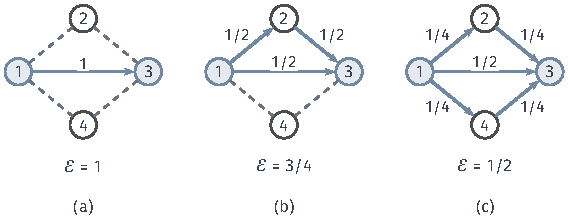
\includegraphics[scale=1]{figures/03-graphs/05-matrices-and-spectra/tikz/electrical-distribution-dissipation/figure.pdf}
  \caption{同一单位注入下的三种分流。顶点$1$注入一单位电流，顶点$3$引出一单位，各边电阻都为一。箭头和数值给出有流量的边，虚线为零电流的边。(a)~只走对角边，(b)~平分到对角边和上路，(c)~网络的实际分流。}
  \label{fig:electrical-distribution-dissipation}
\end{BookInlineFigure}

\paragraph{与最小费用流的比较}

第~\ref{chap:min-cost-flow}章的最小费用流也在守恒条件下选流量，但目标函数是线性的，通常还有容量约束。这里的耗散是严格凸的二次函数，不存在容量限制，边流可以取任意实数。正因为严格凸，极小点唯一——不需要另外检查是否有多个最优解。即使注入量为整数，最优的边流量也可能是分数，如本例中的$1/4$和$1/2$。
